\documentclass[12pt,letterpaper]{article}
\usepackage[utf8]{inputenc}
\usepackage[spanish]{babel}
\usepackage{graphicx}
\usepackage[left=2cm,right=2cm,top=2cm,bottom=2cm]{geometry}
\usepackage{graphicx} % figuras
% \usepackage{subfigure} % subfiguras
\usepackage{float} % para usar [H]
\usepackage{amsmath}
%\usepackage{txfonts}
\usepackage{stackrel} 
\usepackage{multirow}
\usepackage{enumerate} % enumerados
\renewcommand{\labelitemi}{$-$}
\renewcommand{\labelitemii}{$\cdot$}
% \author{}
% \title{Caratula}
\begin{document}

% Fancy Header and Footer
% \usepackage{fancyhdr}
% \pagestyle{fancy}
% \cfoot{}
% \rfoot{\thepage}
%

% \usepackage[hidelinks]{hyperref} % CREA HYPERVINCULOS EN INDICE

% \author{}
\title{Caratula}

\begin{titlepage}
\begin{center}
\large{UNERSIDAD PRIVADA DE TACNA}\\
\vspace*{-0.025in}
\begin{figure}[htb]
\begin{center}

\includegraphics[width=7cm]{./Imagenes/logo}
\end{center}
\end{figure}
\vspace*{0.15in}
INGENIERIA DE SISTEMAS  \\

\vspace*{0.3in}
\begin{large}
\textbf{TITULO:} \\
\end{large}

\vspace*{0.1in}
\begin{Large}
\textbf{Business Intelligence vs. Business Analytics} \\

\end{Large}

\vspace*{0.3in}
\begin{Large}
\textbf{CURSO:} \\
\end{Large}

\vspace*{0.1in}
\begin{large}
INTELIGENCIA DE NEGOCIOS\\
\end{large}

\vspace*{0.3in}
\begin{Large}
\textbf{DOCENTE(ING):} \\
\end{Large}

\vspace*{0.1in}
\begin{large}
 Patrick Cuadros Quiroga\\
\end{large}

\vspace*{0.4in}
\vspace*{0.1in}
\begin{large}
\textbf{INTEGRANTE:} \\
\begin{flushleft}
Zavala Venegas, Luis Angel	\hfill	(2010037899)\\
Condori Quiso, Jesus		\hfill	(2008032440)\\
Condori Tito, Hernan		\hfill	(2009034553)\\
Vilca Chambilla, Wilfredo		\hfill	(2006028540)\\
Vilca Mamani, Elisban		\hfill	(2013000787)


\centering  %CENTRA UN TEXTO
\vspace*{0.9in}
\begin{large}
Tacna\\ 26-10-2018
\end{large}


\end{flushleft}
\end{large}
\end{center}

\end{titlepage}


\tableofcontents % INDICE
\thispagestyle{empty} % INDICE SIN NUMERO
\newpage
\setcounter{page}{1} % REINICIAR CONTADOR DE PAGINAS DESPUES DEL INDICE


\section{Introdución} 
\vspace{12mm} %5mm vertical space


Los analistas de negocios y los compradores de software a menudo preguntan cuáles son las diferencias clave entre la inteligencia empresarial frente al análisis comercial.

Las soluciones de inteligencia empresarial se encuentran entre las herramientas de gestión de datos más valiosas disponibles. Las soluciones de BI recopilan y analizan datos actuales y procesables con el fin de proporcionar información para mejorar las operaciones comerciales. ¿Está buscando formas de comprender mejor sus operaciones comerciales? ¿Qué pasa con descubrir puntos de dolor en sus flujos de trabajo? ¿Qué hay de analizar conjuntos de datos grandes para extraer conocimientos valiosos? Necesita una solución de inteligencia empresarial.

El software de análisis de negocios es un niño o un padre (dependiendo de a quién se lo pregunte) de la categoría de inteligencia empresarial. Al igual que BI, se usa principalmente para analizar datos históricos, pero con la intención de predecir tendencias comerciales. También generalmente tiene un ojo hacia la mejora y la preparación para el cambio.

Las organizaciones están empezando a ver que los datos y el contenido no deben considerarse aspectos separados de la gestión de la información, sino que deben gestionarse en un enfoque empresarial integrado. Muchas empresas se están moviendo hacia la inteligencia comercial operativa, que actualmente no cuenta con los proveedores adecuados.
Si bien es superficialmente similar, la diferencia entre BI y BA es clara una vez que se hace una pequeña excavación.

		


\section{Business Intelligence} 
\vspace{16mm} %5mm vertical space
\begin{center}

\includegraphics[width=10cm]{./Imagenes/001}
\end{center}	
\vspace{12mm} %5mm vertical space

El término se refiere a tecnologías, aplicaciones y prácticas para la recopilación, integración, análisis y presentación de información comercial. El objetivo de la inteligencia empresarial es apoyar la toma de decisiones comerciales basadas en datos. La inteligencia empresarial a veces se usa indistintamente con libros de instrucciones, herramientas de informes y consultas, y sistemas de información ejecutiva.

BI mejora y mantiene la eficiencia operativa y ayuda a las empresas a aumentar la productividad de la organización. El software de inteligencia empresarial ofrece muchos beneficios, que incluyen poderosas funciones de generación de informes y análisis de datos. Al utilizar los mecanismos de visualización de datos de BI, como los paneles de control en tiempo real, los gerentes pueden generar informes intuitivos y legibles que contienen datos relevantes y procesables.

Entonces BI ofrece informes y análisis, ¿no son solo dos palabras para lo mismo? Muchas personas, tanto dentro como fuera de la industria del software, usan información y análisis de forma incorrecta, lo que es una de las causas de la confusión detrás de la combinación BA / BI.\\

\textbf{Informes} es el proceso de organizar datos en resúmenes informativos con el fin de monitorear cómo se desempeñan las diferentes áreas de un negocio". Recopila datos y los entrega en un formato digerible.\\

\textbf{Analytics} es el proceso de explorar datos e informes con el fin de extraer ideas significativas, que pueden usarse para comprender mejor y mejorar el rendimiento comercial". Esta función toma el "qué" de los datos proporcionados por los informes y saca conclusiones y perspectivas, ofreciendo los usuarios un "por qué" y "cómo". Básicamente, las funciones de informe presentan datos y las funciones de análisis interpretan los datos. Ambas son características cruciales y, por lo general, las soluciones de BA y BI las ofrecerán.
	



\section{Business Analytics} 

\vspace{16mm} %5mm vertical space
\begin{center}

\includegraphics[width=17cm]{./Imagenes/002}
\end{center}	
\vspace{12mm} %5mm vertical space

Al igual que la inteligencia empresarial, BA recopila y analiza datos, emplea el análisis predictivo y genera informes ampliamente visualizados en tableros personalizados. El objetivo de estas características es ayudar a identificar y abordar los puntos débiles de una organización. Aquí es donde terminan las similitudes. El software de análisis empresarial se utiliza para explorar y analizar datos históricos y actuales. Utiliza el análisis estadístico, la minería de datos y el análisis cuantitativo para identificar las tendencias comerciales pasadas.\\
Una vez que se han recopilado y analizado los datos, los sistemas de análisis de inteligencia empresarial luego usan esa información para el modelado predictivo. Esto puede predecir y, en la mayoría de los casos, prepararse para los climas comerciales futuros. Uno de los aspectos más potentes de BA es la generación de informes ad hoc, que permite a las empresas realizar análisis de datos específicos en tiempo real para responder preguntas específicas y tomar decisiones comerciales más rápidas. En efecto, el análisis empresarial usa el análisis predictivo para resolver problemas antes de que ocurran.\\
BA es una expresión general para los enfoques y las tecnologías que puede utilizar para acceder y explorar los datos de su empresa, con el fin de extraer nuevos conocimientos útiles para mejorar la planificación empresarial y aumentar el rendimiento futuro.


\section{Business Intelligence vs. Business Analytics: ¿Cuál es la diferencia?} 
\textbf{Elegir entre Business Intelligence y Business Analytics}
\vspace{5mm} %5mm vertical space

Las organizaciones están empezando a ver que los datos y el contenido no deben considerarse aspectos separados de la gestión de la información, sino que deben gestionarse en un enfoque empresarial integrado. Muchas empresas se están moviendo hacia la inteligencia comercial operativa, que actualmente no cuenta con los proveedores adecuados.\\

\vspace{5mm} %5mm vertical space
\begin{center}
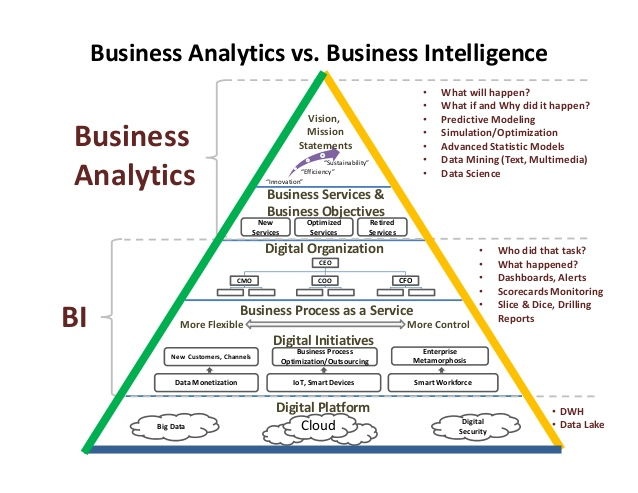
\includegraphics[width=14cm]{./Imagenes/003}
\end{center}	
\vspace{12mm} %5mm vertical space

\textbf{Evalúa tus necesidades} Tradicionalmente, los proveedores de inteligencia empresarial se enfocaban principalmente en las empresas, pero ahora hay un cambio de paradigma de que BI se mude a las pequeñas y medianas empresas. El autoservicio de BI es un enfoque principal de estas compañías más pequeñas.

La inteligencia empresarial de autoservicio (SSBI) es un enfoque para el análisis de datos que permite a los usuarios acceder y trabajar con datos corporativos aunque no tengan experiencia en análisis o ciencia de datos. Por lo general, cuenta con una interfaz de usuario más amigable y no implica codificación, por lo que su joe regular puede operarlo.\\


\textbf{Elija con Intención} Elegir la solución para su negocio depende de sus intenciones. Si está satisfecho con su modelo de negocio en general y desea principalmente mejorar las operaciones, aumentar la eficiencia y cumplir los objetivos de la organización, la inteligencia empresarial puede ser una solución óptima. En particular, las empresas que confían en los informes en tiempo real tienden a inclinarse hacia 
BI, ya que están preocupados por lo que pueden mejorar aquí y ahora.

Por otro lado, si tiene la intención de cambiar los procesos de su empresa, o incluso su modelo de negocio completo, pero todavía no tiene los conocimientos necesarios, el análisis de negocios podría ser la mejor opción.

Las empresas que requieren una gran cantidad de datos (por ejemplo, la necesidad de almacenamiento de datos) e informes intuitivos deben considerar seriamente la inteligencia empresarial. BI tiene las ventajas adicionales de dirigirse a las áreas débiles de una empresa y proporcionar información accionable sobre esos problemas. Las herramientas de inteligencia comercial son excelentes soluciones para los gerentes que desean mejorar la toma de decisiones y comprender la productividad, los procesos de trabajo y los empleados de su organización. Luego, con esa comprensión, mejore su negocio desde cero.


\section{Perspectivas de expertos} 

Encuestamos a siete expertos líderes en todo el espectro de inteligencia empresarial para comprender mejor la distinción entre estos dos términos de referencia.
\vspace{6mm} %5mm vertical space

\textbf{Mantener vs. revolucionar}
Se necesita Business Intelligence para administrar el negocio, mientras que Business Analytics es necesario para cambiar el negocio.
BI se enfoca en crear eficiencia operativa a través del acceso a datos en tiempo real que permiten a las personas realizar de manera más efectiva sus funciones de trabajo.\\ BI también incluye el análisis de datos históricos de múltiples fuentes que permiten una toma de decisiones informada, así como la identificación y resolución de problemas.\\Business Analytics se relaciona con la exploración de datos históricos de muchos sistemas fuente a través del análisis estadístico, análisis cuantitativo, minería de datos, modelado predictivo y otras tecnologías y técnicas para identificar tendencias y comprender la información que puede impulsar el cambio comercial y respaldar prácticas comerciales exitosas sostenidas.
\begin{flushleft}
Pat Roche\\  
Vicepresidente de Ingeniería, Noetix Products\\  
Magnitude Software
\end{flushleft}

\textbf{Comprender el pasado versus el futuror}
Para mí, la diferencia entre Business Intelligence es mirar por el espejo retrovisor y usar datos históricos desde hace un minuto hasta hace muchos años. Business Analytics está mirando en frente de usted para ver qué va a pasar. Esto te ayudará a anticipar lo que viene, mientras que BI te dirá lo que sucedió. Esta es una distinción muy importante ya que ambos le proporcionarán diferentes puntos de vista, no menos. La BI es importante para mejorar su toma de decisiones sobre la base de resultados pasados, mientras que los análisis de negocios le ayudarán a avanzar y comprender lo que podría suceder.
\begin{flushleft}
Mark van Rijmenam\\  
CEO / Fundador\\  
BigData-Startups
\end{flushleft}

\textbf{Informes y análisis}
La inteligencia empresarial tradicional (BI) se ha centrado principalmente en la elaboración de informes. En este enfoque de BI, algunas personas crean informes con muchos formatos (por lo general, los desarrolladores de informes) y se distribuyen a todo un departamento u organización. Más recientemente, la tendencia en análisis ha sido brindar a las personas que tienen preguntas sobre sus datos las herramientas para obtener sus propias respuestas. Ahora se trata de dejar que las personas de negocios se conviertan en analistas.\\ Esto a menudo se conoce como "análisis de autoservicio", y en este enfoque no se trata solo de generar informes, sino de permitir que las personas entren en el flujo del análisis, exploren sus datos y formulen sus propias preguntas. Esto ha cambiado por completo la forma en que muchas empresas se acercan a la inteligencia de negocios.
\begin{flushleft}
Francois Ajenstat \\  
Tableau
\end{flushleft}
\section{Conclusiones} 

Business intelligence nos permite visualizar y hacer análisis en base a la información histórica,  es decir hacia el pasado nos brinda tendencia de como se ha desarrollado historicamente el negocio de una compañia, pero hoy en dia eso no lo es todo ya que se necesita tambien analizar el futuro y eso es lo que se llama Business analytics nos permite  poder predecir en base a la experiencia en base a la información que se tiene,  en base a  modelos predictivo y anticiparse a lo que otras compañias  desconocen, es la gran diferencia una mira la pasado y otra al futuro con modelos predictivos.






\end{document}
